\documentclass[a4paper, 12pt, french, twoside]{article}
\usepackage{graphicx,wrapfig,lipsum}
\usepackage{graphicx}
\usepackage{mathtools}
\usepackage{amsmath}
%\frenchbsetup{StandardLists=true} à inclure si on utilise 
\usepackage[french]{babel}
\usepackage{enumitem}
\usepackage{float}
%\usepackage[top=2.5cm, bottom=2cm, left=2cm, right=2cm, showframe]{geometry}
\usepackage[top=2.5cm, bottom=2cm, left=2cm, right=2cm]{geometry}
\usepackage{caption}
\usepackage{amsmath}
\usepackage{graphicx} % Required for inserting images
\usepackage{subcaption}
\usepackage{hyperref}
\usepackage{makecell}
\usepackage{amsfonts}
\usepackage{amsthm}


\newtheorem{theorem}{Théorème}[section]
\newtheorem{corollary}{Corollaire}[theorem]
\newtheorem{lemma}[theorem]{Lemme}
\newtheorem{proposition}{Proposition}[theorem]
\newtheorem{defi}{Définition}[theorem]
\newtheorem{rem}{Remarque}[theorem]

\usepackage{pdfpages} % lien Pdf test
 \usepackage{tcolorbox}

\usepackage{cleveref}
\crefrangelabelformat{equation}{(#3#1#4--#5#2#6)}
\crefname{equation}{Eq.}{Eqs.}
\Crefname{equation}{Equation}{Equations}


%\usepackage{movie15}
\usepackage{epstopdf}
\usepackage{subcaption}
\usepackage{multicol}

%a abréviations
\def \be {\begin{equation}}
\def \ee {\end{equation}}
\def \dd  {{\rm d}}
\def \bm {\begin{pmatrix}}
\def \em {\end{pmatrix}}

%Ensembles 
\newcommand{\Cc}{{\mathbb{C}}}
\newcommand{\Ct}{\Cc^\times}
\newcommand{\Hh}{{\mathbb{H}}}
\newcommand{\Nn}{{\mathbb{N}}}
\newcommand{\Zz}{{\mathbb{Z}}}
\newcommand{\Zzn}{\Zz/n\Zz}
\newcommand{\ZzNt}{(\Zz/N\Zz)^\times}%quotient 
\newcommand{\Rr}{{\mathbb{R}}}
\newcommand{\Rt}{{\Rr^\times}}
\newcommand{\Qt}{{\Qq^\times}}
\newcommand{\Qq}{{\mathbb{Q}}}
%to do later
\newcommand{\later}[1]{\textcolor{orange}{[#1]}}
\newcommand{\com}[1]{\textcolor{magenta}{[#1]}}

%to make hyper refs not surrounded with red
\hypersetup{pdfborder=0 0 0}
\hypersetup{
    colorlinks=true,
    linkcolor=blue,
    filecolor=magenta,      
    urlcolor=cyan,
    pdftitle={Overleaf Example},
    pdfpagemode=FullScreen,
    }
    
\title{Série 1}

\begin{document}

\maketitle



\section{Ex 1}
Montrer que si $a^2$ est pair, alors $a$ est pair.

\section{Ex 2}
Soit les ensembles suivants: $A$=\{0,4,8,3\}, $B$=\{3, 7, 9\}, $C$=(0,1], $D$=(0.5, 2].
Trouvez:

\begin{enumerate}
    \item $A\cup B$
    \item $A \cap B$
    \item $C\cup D$
    \item $C\cap D$
    \item $A\cap C$
    \item $A\cup C$
\end{enumerate}

\section{Ex 3}
Montrer par récurrence la formule explicite des suites arithmétiques et géométriques en partant des définitions par récurrence suivantes:
\begin{equation}
    \begin{cases}
        x_{n+1}=x_n+r, ~~\text{arithmétique}\\
        x_{n+1}=x_n\cdot r, ~~\text{géométrique}
    \end{cases}
\end{equation}


\section{Convergence de suite, suite monotone bornée}
Le présent exercice a pour but d'étudier la convergence d'une suite de deux manières:
\begin{enumerate}
    \item En utilisant la définition de limite d'une suite (méthode générale, applicable à toute suite convergente);
    \item En utilisant le théorème des suites monotones bornées, après avoir vérifié que la suite est (dé)croissante et bornée supérieurement (inférieurement).
\end{enumerate}

Voici l'expression de la suite considérée:
\begin{equation}
    x_n = \frac{n}{n+1} \quad \forall n\in \Nn
    \label{exo_suite_limite}
\end{equation}

\subsection{Méthode 1: Par la définition}
\textbf{a)} Afin de mieux visualiser la suite, commencez par représenter quelques-uns de ses points sur le graphique de la Figure \ref{fig:exo4.1a} (réflexe à avoir si vous ne visualisez pas trop une suite!). \\

\begin{figure}[H]
    \centering
    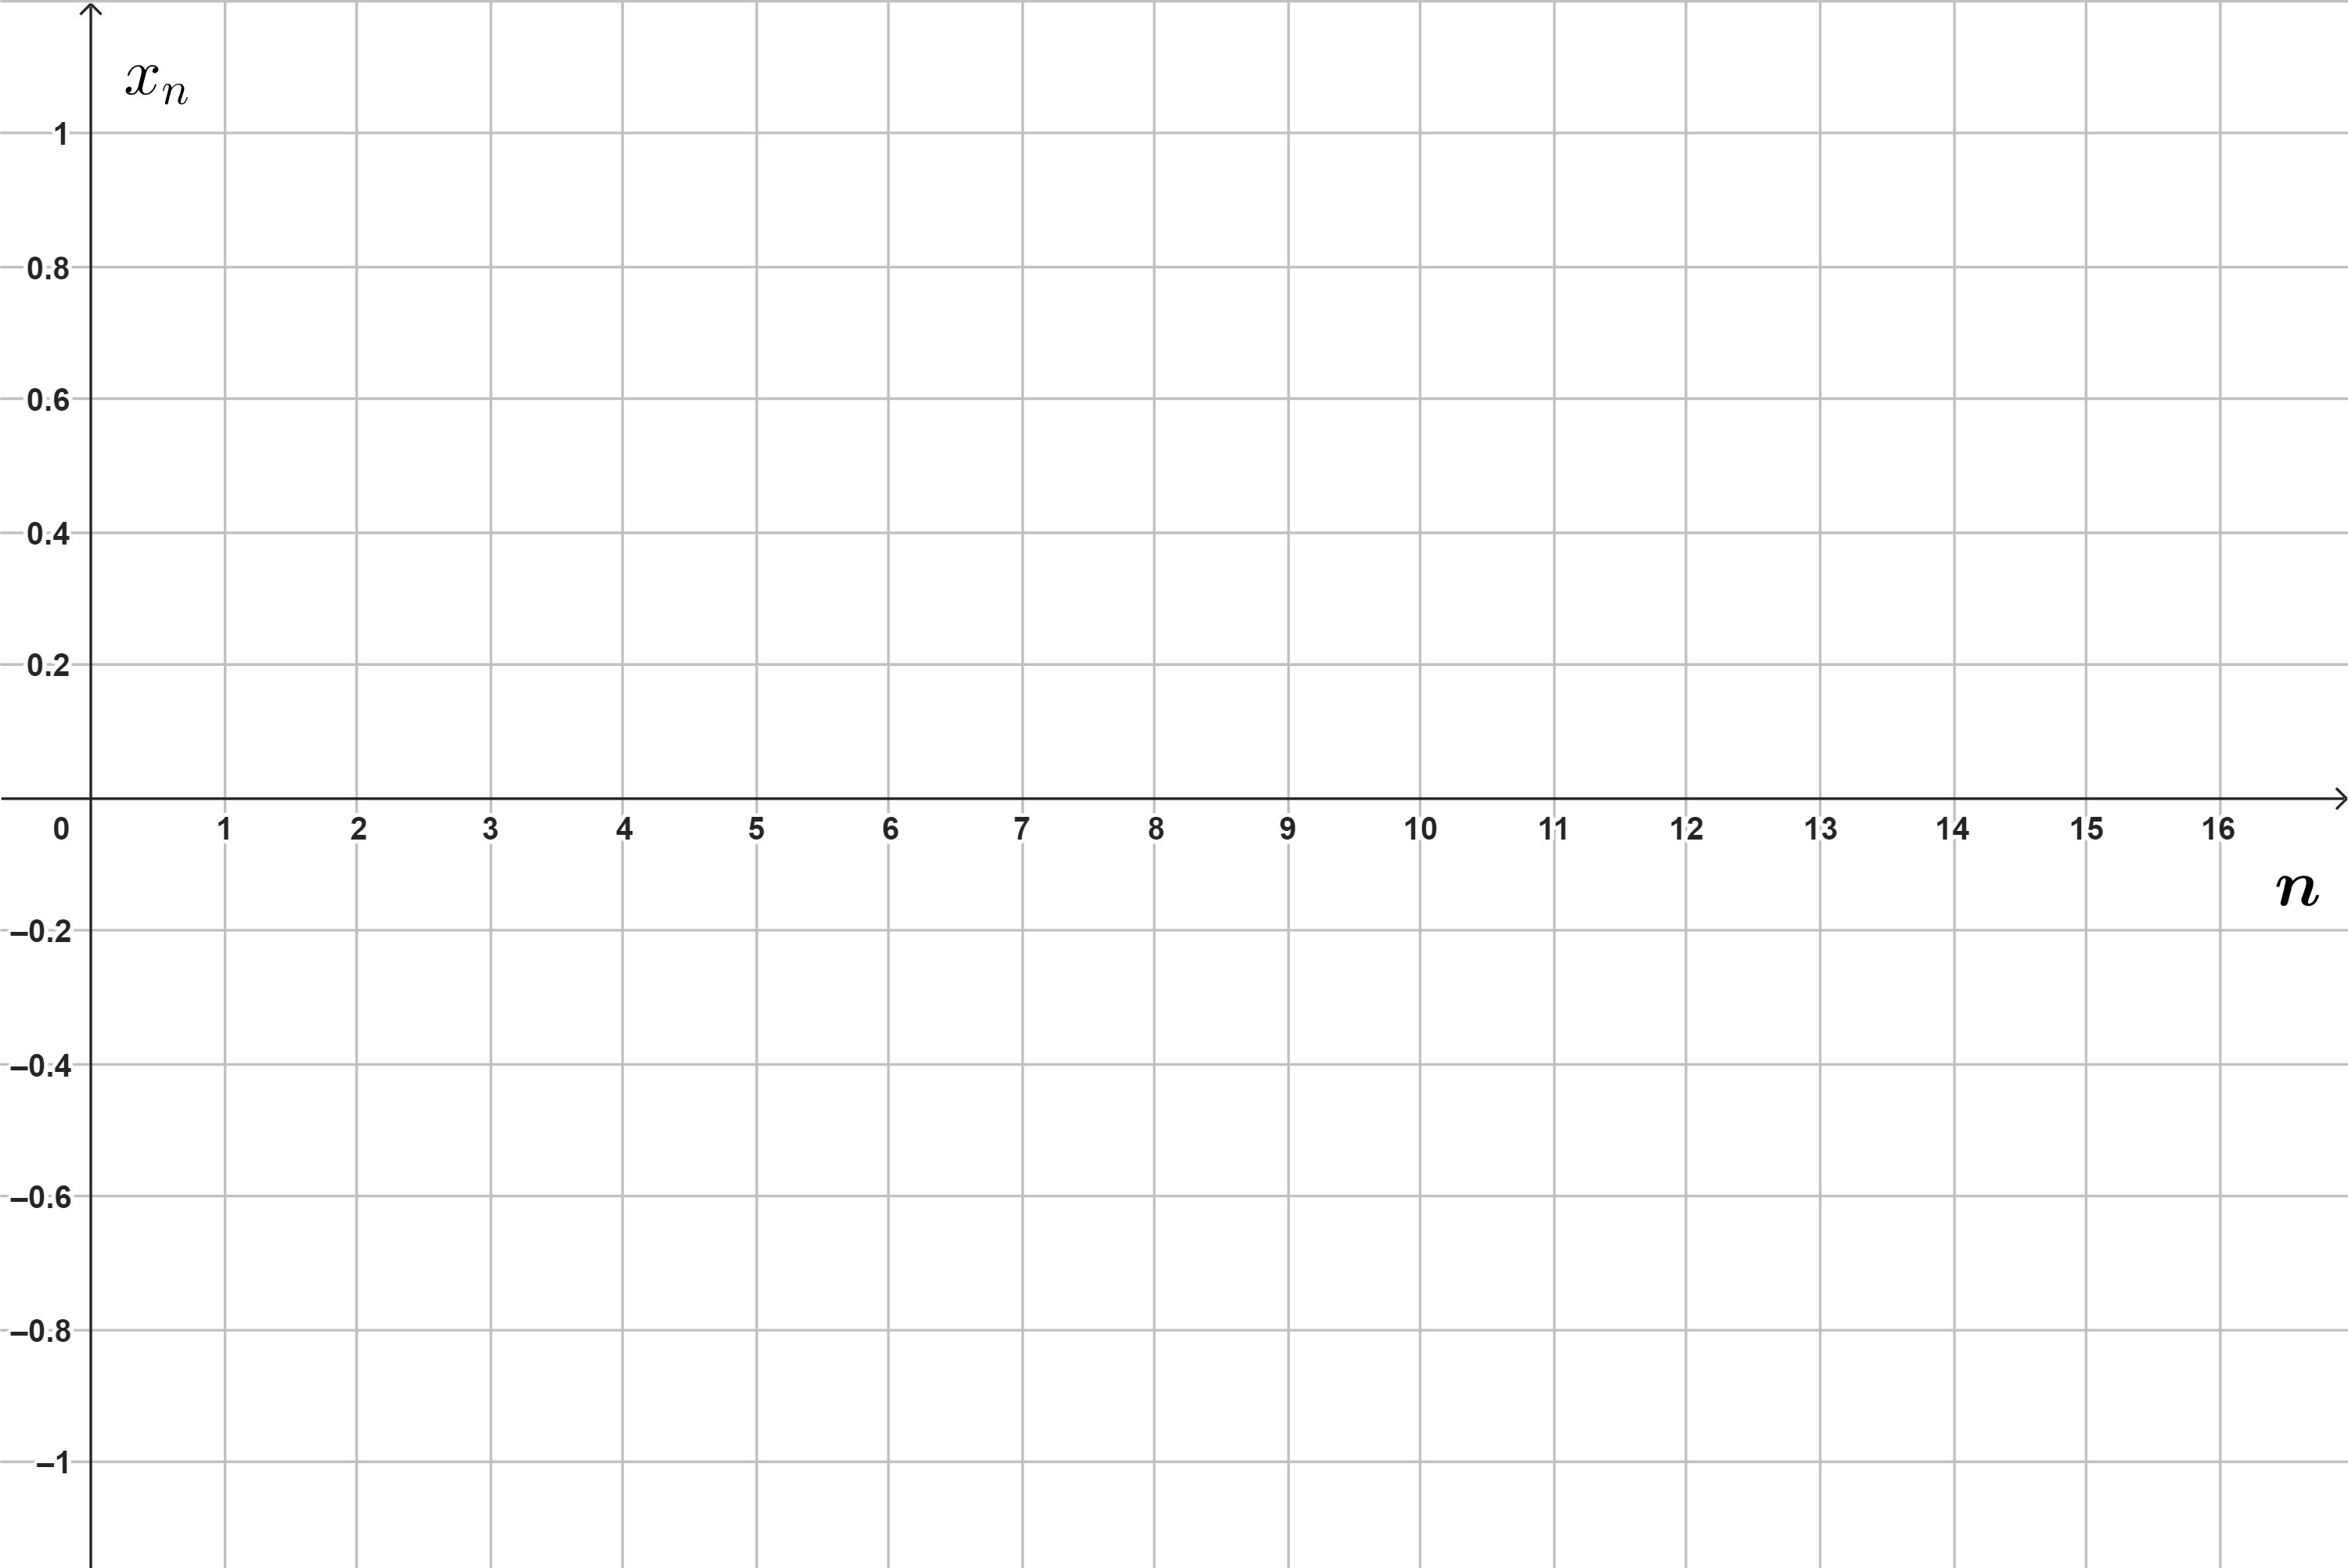
\includegraphics[scale=0.8]{Exercices/exo_sabri.png}
    \caption{Exercice \textbf{4.1 a)}}
    \label{fig:exo4.1a}
\end{figure}\\

\textbf{b)} Vers quelle limite cette suite converge-t-elle (pas besoin d'utiliser la définition à ce stade)? \\

\textbf{c)} Pour rappel, la définition de limite de suite nous dit que quelque soit l'erreur $\epsilon$ souhaitée, aussi petite soit-elle, il existe un moment dans la suite (un naturel $N$) à partir duquel l'écart entre la suite et sa limite est inférieur à l'erreur $\epsilon$.\\ 
Trouvez le plus petit naturel $N$ satisfaisant cette condition si on choisit comme erreur $\epsilon = 0.1$. \\ \textbf{Indice:} Aidez-vous de votre graphique en Figure \ref{fig:exo4.1a}.\\

\textbf{d)} Généralisons la démarche du point \textbf{c)}: trouvez la condition que le naturel $N$ de la définition de limite doit satisfaire pour que l'erreur soit de $\epsilon$.\\
\textbf{Indice:} Vous devriez obtenir une inégalité de la forme $N > f(\epsilon)$, où $f$ est une fonction.\\

\faLightbulbO \quad \fbox{\textbf{Discutez}} Comment l'exercice change-t-il lorsque l'on considère la suite suivante?
\begin{equation}
    y_n = \frac{n^2}{n+1} \quad \forall n\in \Nn
\end{equation}

\subsection{Méthode 2: Par le théorème des suites monotones bornées}
\textbf{a)} Montrez que la suite \eqref{exo_suite_limite} est bornée supérieurement. Quel est son suprémum? Ce suprémum est-il un maximum (pas nécessaire pour utiliser le théorème, mais c'est bien de comprendre la distinction entre suprémum et maximum)?\\

\textbf{b)} Montrez que la suite est croissante.\\

\textbf{c)} Le théorème des fonctions monotones bornées vous permet de conclure que la suite converge (vers son suprémum, car fonction croissante dans ce cas-ci). \\ Prouvez ce théorème de manière générale pour les fonctions croissantes bornées supérieurement.\\
\textbf{Indice:} Commencez par formaliser la notion de suprémum en utilisant l'erreur $\epsilon$ (similaire à la définition de limite: ``$\forall \epsilon ...$''). Combinez avec la notion de croissance, puis concluez.\\

\faLightbulbO \quad \fbox{\textbf{Discutez}} Le théorème des suites monotones bornées est très pratique pour étudier la convergence de suites définies par récurrence, comme par exemple:
\begin{equation}
    x_0 = 0.5, \quad x_{n+1} = \frac{x_n + 1}{2} \quad \forall n\in \Nn
\end{equation}
Comment feriez-vous pour prouver que cette suite est bornée supérieurement(inférieurement)/\\ (dé)croissante?


\end{document}
